\section{Problem 5}~\label{sec:prob5}

\subsection{} % 5.1

\begin{figure}[ht]
\centering
    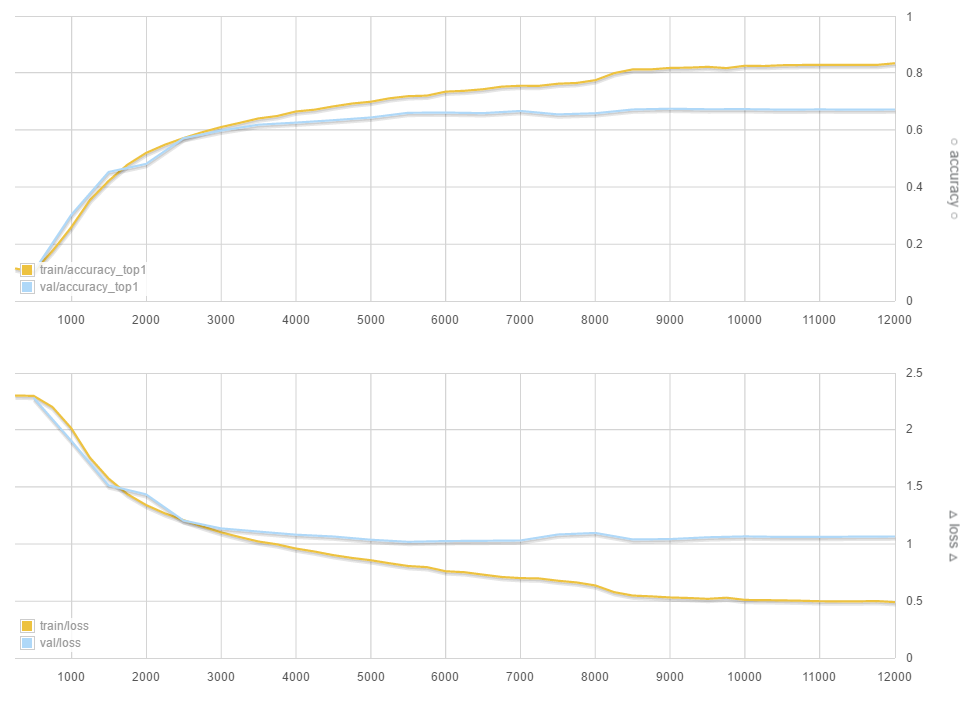
\includegraphics[width=0.99\linewidth]{fig/curve1}
    \caption{\small
    Training curve of the simple network on CIFAR-10.
    initialization is Gaussian.
    The batch size is 256.
    Use SGD as described in the problem.
    The step sizes are 8000, 10000 and 12000.}
    \label{fig:1}
\end{figure}

\subsection{} % 5.2

Since $w_l$ has zero mean,
so does $w_l x_l$.
Together with independence between $x_l$ and $w_l$,
we have

\begin{equation}
\begin{split}
    \Var[y_l] &= n_l \Var[w_l x_l] \\
        &=n_l E[w_l^2 x_l^2] - 0 \\
        &=n_l E[w_l^2] E[x_l^2] \\
        &=n_l \Var[w_l] E[x_l^2].
\end{split}
\end{equation}

To prove $E[x_l^2]=Var[y_{l-1}]/2$,
we need assume that $y_{l-1}$ is Gaussian with zero mean.
Since
\begin{equation}
    x_l = \begin{cases}
        y_l, &\text{ if }y_l\ge0\\
        0, , &\text{ if }y_l<0\\
    \end{cases}
\end{equation}
So
\begin{equation}
    E[x_l^2] = \int_0^\infty p(x_l)x_l^2 dx_l
        = \frac{1}{2}\int_{-\infty}^\infty p(x_l)x_l^2 dx_l
        = \frac{1}{2}Var[y_{l-1}].
\end{equation}

The initialization described here is the \emph{msra} initialization~\cite{he2015delving}.

\subsection{} % 5.3

\subsection{} % 5.4
